\chapter{A Space-time \Skewt Model for Threshold Exceedances}
\chaptermark{Space-time \Skewt Model}
\label{chap:two}

\section{Introduction}\label{sts:intro}
% In many climatological applications, researchers are interested in learning about the average behavior of different climate variables (e.g. ozone, temperature, rainfall).
Epidemiological studies have linked air quality to public health concerns regarding morbidity and mortality \citep{Samet2000}.
As a result, the Environmental Protection Agency (EPA) has developed a set of standards to help reduce air pollution thereby improving air quality.
Our study is motivated by an air pollution application where the focus is not on the average behavior, but on the behavior over a high level determined by government regulation.
More specifically, we consider the case of compliance for ozone.
A site is said to be in compliance if the fourth highest daily maximum 8-hour concentration averaged over three years does not exceed 75 parts per billion (ppb).
\fref{stfig:ozone-10jul} shows the ozone levels from July 10, 2005, at 1089 stations across the United States.
We see a large area above the compliance level in the midwest covering Ohio, Indiana, Illinois, and parts of the surrounding states.
We analyze these data with the goals of spatial prediction for unmonitored locations and to map the probability of extreme events.

\begin{figure}[h!tbp]
  \centering
  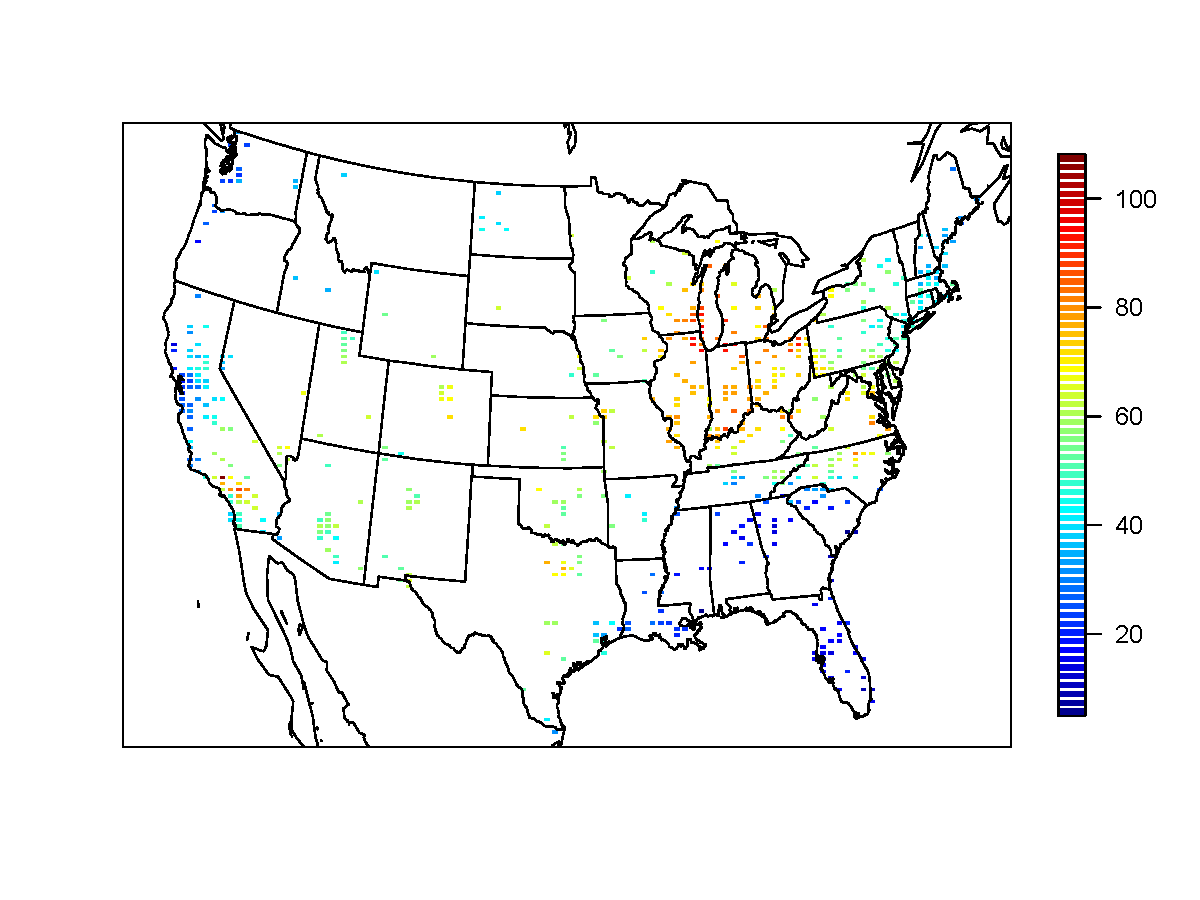
\includegraphics[width=0.75\linewidth]{plots/ozone-10jul-us.pdf}
  \caption{Ozone values (ppb) on July 10, 2005}
  \label{stfig:ozone-10jul}
\end{figure}

A spatial model for threshold exceedances warrants special consideration and standard spatial methods are likely to perform poorly.
First, because we are interested only in high values, we want to ``let the tail speak for itself''.
That is, if we fit a model to the entire data set, low-to-moderate values would influence the fit of the overall model.
As there are more of these values, they can unduly influence the distribution at the higher levels about which we are interested.
Our inference method will only use data which exceed a pre-selected threshold and will censor data below the threshold, thereby tailoring the fit to the levels of interest.
Second, likelihood-based spatial modeling typically assumes a Gaussian process, which is appropriate when mean behavior is of interest.
However, the Gaussian distribution is light-tailed and symmetric, and therefore may be inappropriate for modeling data which does not share this tail behavior.
Third, we aim to capture the dependence structure when ozone is at high levels, and dependence at these levels may not be well-represented by covariances which focus again on mean behavior.
Asymptotic dependence/independence (see \sref{sts:extdep}) are notions which describe how two random variables' probability of simultaneous exceedance of an extremely high level.
The Gaussian distribution always exhibits asymptotic independence, except in the case of perfect dependence, thus is an inappropriate model for data which exhibits asymptotic dependence.
To allow for more flexibility in the marginal tail and to allow for asymptotic dependence, the \skewt distribution forms the basis for our model.

Our approach differs from threshold modeling approaches based on extreme value distributions.
There has been extensive work on threshold modeling in the field of extreme value statistics where extreme events are naturally defined in terms of exceedances over a high threshold.
\citet{Davison1990} considered modeling threshold exceedances of univariate time series by the generalized Pareto distribution.
Threshold based inference for multivariate extreme value distributions was considered by \citet{Ledford1996} who introduced a censored approach that provides a way to deal with different types of exceedances of a threshold.
These models were extended to spatial models for threshold exceedances by \citet{Wadsworth2012} and \citet{Thibaud2013} who fit various models to spatial extremes using a censored pairwise likelihood \citep{Padoan2010} based on the approach of \citet{Ledford1996}.
\citet{Huser2014} further extended this to space-time modeling.
\citet{Wadsworth2014}, \citet{Engelke2015}, and \citet{Thibaud2013a} introduced more efficient inference for threshold exceedances of extremal spatial processes with full likelihood methods.
The previous approaches to threshold modeling are motivated by extreme value theory and assume the threshold is high enough that extremal models are valid for the data and for extrapolation beyond the range of observed values.
Moreover, these approaches are computationally intensive and limited to rather small datasets.
% For example, \citet{Wadsworth2014} present a simulation study with observations at 16 sites on a regular grid, and \citet{Engelke2015} analyze a dataset with observations at 35 meteorological stations.
Our application with ozone data does not fit into this framework because we do not focus on exceedances of a very high level, and we have observations at 1,089 ozone monitoring locations.

We propose a new spatiotemporal threshold exceedance model based on the \skewt process \citep{Padoan2011}.
We use a \skewt distribution because of its flexibility to model asymmetry and heavy-tailed data with the aim of modeling exceedances of a high fixed level at an unobserved location.
Our model allows for inference and predictions using the full likelihood with computing on the order of Gaussian models.
This allows us to use Bayesian methods, which we use to fit the model, handle censored data below the threshold, and make predictions at unobserved locations.
The multivariate skew normal distribution was introduced by \citet{Azzalini1996}, and this was extended to the multivariate \skewt by \citet{Branco2001}.
These skew-elliptical distributions have been used in the spatial setting \citep{Genton2004,Kim2004}.
\citet{Zhang2010} propose the skew-Gaussian process as a class of stationary processes that have skewed marginal distributions.
\citet{Padoan2011} examined the usage of skew-Gaussian and \skewt distributions for multivariate extremes.
In a spatial setting, the multivariate \skewt distribution demonstrates asymptotic dependence between observations at all sites regardless of the distance between the sites.
In order to address this concern, we introduce a random spatial partition similar to the method used by \citet{Kim2005} for non-stationary Gaussian data.
% This partitioning alleviates the asymptotic spatial dependence present in the \skewt distribution for sites that are far apart.

The paper is organized as follows.
\sref{sts:spatialskew} is a brief review of the spatial \skewt process.
In \sref{sts:spatial}, we build upon the traditional \skewt process by incorporating censoring, partitioning, and extending the model to space-time data.
The computing is described in \sref{sts:hier}.
In \sref{sts:simstudy}, we present a simulation study that examines the predictive capabilities of this model compared to Gaussian and max-stable methods.
We compare our method to Gaussian and max-stable methods with a data analysis of ozone measurements throughout the US in \sref{sts:analysis}.
% The final section provides brief discussion and direction for future research.

% These models describe dependence using the probability that two observations jointly exceed an extreme value, which in the limit of the distribution is referred to as asymptotic dependence.
% When the spatial domain is small, it may be reasonable to assume that all sites are asymptotically dependent; however for large spatial domains, it becomes more challenging to justify this assumption.
% This concern has been addressed by \citet{Wadsworth2012} in a spatial only setting and \citet{Huser2014} in a space-time setting.

% The main goal of our application is to estimate the marginal probability a site's ground-level ozone measurement will exceed 75 ppb.
% For July 2005, 75 ppb is approximately the 92nd sample quantile.
% However, if we look marginally at each site, 75 ppb is lower than the 90th quantile for almost 255 sites, and is below the median at 29 sites.
% The traditional threshold exceedance models arising from max-stable processes incorporate thresholding because the inference is only valid for very high values.
% Because 75 ppb represents such a wide range of marginal quantiles, these models based on max-stable methods may not be appropriate.

% Traditionally, spatial methods for extreme values analysis are conducted from one of two perspectives.
% The first of these is based on the convergence of the maximums of independent stochastic processes to a max-stable process \citep{deHaan2006}.
% Finite dimensional realizations of a max-stable process follow a generalized extreme value distribution \citep{Cooley2012}.
% One drawback to a block-maxima approach is that information is lost by discarding all but the most extreme observations in a block.
% Furthermore, in using multivariate block-maxima methods, the observations in the vector of block maxima rarely occur simultaneously \citep{Coles2001}.
% The other perspective incorporates a peaks-over-threshold approach.

% The use of multivarate models for threshold exceedances require evaluation of the underlying joint density.
% Finite dimensional realizations of max-stable processes are challenging to use because closed-form expressions for the density in more than two dimensions are complicated \citep{Coles1991}.
% One way to circumvent this challenge is to use pairwise composite likelihood methods \citep{Padoan2010}.
% When using pairwise composite likelihoods, threshold methods can then be implemented as long as the bivariate distribution can be evaluated \citep{Wadsworth2012,Thibaud2013,Huser2014}.
% Hierarchical models using Bayesian methods have also been proposed.
% For example, \citet{Reich2012} present a Bayesian hierarchical model, when conditioned on positive stable spatial random effects, the observations are independent.

% In certain settings, the multidimensional distributions are available.
% For example, \citet{Wadsworth2014} discuss a censored Poisson process that exploits the fact that the spectral functions for Brown-Resnick processes are log-Gaussian random fields.
% Additionally, \citep{Engelke2014}, show that upon standardizing marginals to the Gumbel distribution and conditioned on a fixed location exceeding a high threshold, the incremental distribution asymptotically forms a Gaussian process.
% In addition to Brown-Resnick processes, skew elliptical distributions can be used for multivariate modeling with dependent extreme values \citep{Genton2004,Zhang2010,Padoan2011}.
% For example, the skew-normal and \skewt distribution offer a flexible way to handle non-symmetric data within a framework of multivariate normal and multivariate $t$ distributions.
% As with multivariate Gaussian distributions, the multivariate skew-normal distribution demonstrates asymptotic independence. Conversely both the multivariate $t$ and \skewt distributions demonstrate asymptotic dependence \citep{Padoan2011}.
% Additionally, the limiting distribution of the maxima of \skewt random vectors is the extremal \skewt distribution \citep{Padoan2011} of which the extremal-$t$ \citep{Opitz2013} is a special case.

% Despite this challenge, spatial modeling is important because it provides a mechanism by which we can borrow information about extreme events across space.
% There are two primary goals for spatial methods.
% The first of these goals is to understand the marginal behavior at sites, and the second is to describe the dependence in the data.
% In many cases, these are done separately; however, with the development of pairwise composite likelihoods and Bayesian methods, it is resonable to model both simultaneously.
% One challenge to estimating the dependence in the tails of the distribution is that the dependence that present in the data may not be the same as the dependence in the limit of the underlying distribution \citep{Davison2012b}.
% Furthermore, in a spatial setting, it may be desirable to allow for varying degrees of tail dependence based upon the distance between two sites \citep{Wadsworth2012}.

\section{Spatial skew processes}\label{sts:spatialskew}
\sectionmark{Spatial skew processes}
The skew-elliptical family of distributions provides models that are mathematically tractable while introducing a slant parameter to account for asymmetric data.
A brief review of the additive process \citep[p. 129]{Azzalini2014} by which a \skewt process is created is given here.

\subsection{\Skewt process} \label{sts:skewt}
\subsectionmark{\Skewt process}
Let $Y(\bs)$ be a spatial process defined for spatial location $\bs$ in a spatial domain of interest $\calD \in \mathbb{R}^2$.
The spatial \skewt process can be written as
\begin{align}
  Y(\bs) = \bX(\bs)^\top \bbeta + \lambda \sigma |z| + \sigma v(\bs) \label{steq:fullmodel}
\end{align}
where $\bX(\bs)$ is the observed covariate vector at site $\bs$, $\bbeta$ is the $p$-vector of regression parameters, $\lambda \in \mathbb{R}$ is a parameter controlling skewness, $z \sim N(0, 1)$, $\sigma^2 \sim \mathrm{IG}(a / 2, b / 2)$ is random scale parameter, IG is the distribution function of an inverse gamma random variable, $a$ is the degrees of freedom, $b$ controls the precision of the process, and $v(\bs)$ is a standard Gaussian process with positive definite correlation function $\text{Cor} \left[Y(\bs_1), Y(\bs_2)\right] = \rho(\bs_1, \bs_2)$.
Although any positive definite correlation function could be used, we choose to use the stationary isotropic \Matern correlation with
\begin{align}
  \rho(h) = (1 - \gamma) I(h = 0) + \gamma \frac{ 1 }{ \Gamma(\nu) 2^{ \nu - 1}} \left( \sqrt{2\nu} \frac{ h }{ \varphi } \right)^{\nu} K_{\nu} \left( \sqrt{2\nu} \frac{ h }{ \varphi } \right) \label{steq:matern}
\end{align}
where $I(\cdot)$ is an indicator function, $\varphi > 0$ is the spatial range, $\nu > 0$ is the smoothness, $\gamma \in [0, 1]$ is the proportion of variance accounted for by the spatial variation, $K_\nu$ is a modified Bessel function of the second kind, and $h = || \bs_1 - \bs_2 ||$ is the Euclidean distance between sites $\bs_1$ and $\bs_2$.

For a finite collection of locations $\bs_1, \ldots, \bs_n$, we denote by $\bY = [Y(\bs_1), \ldots, Y(\bs_n)]^\top$ the vector of observations, and the covariate matrix $\bX_{n \times p} = [\bX(\bs_1), \ldots, \bX(\bs_n)]^\top$.
After marginalizing over both $z$ and $\sigma$, using the notation from \citet[p. 176]{Azzalini2014},
\begin{align} \label{steq:stazzalini}
  \bY \sim \text{ST}_n(\bX \bbeta, \bOmega, \balpha, a),
\end{align}
that is, $\bY$ follows an $n$-dimensional \skewt distribution with location $\bX \bbeta \in \mathbb{R}^n$; covariance matrix $\bOmega_{n \times n} = \bomega \left[ \frac{1}{1 + \lambda^2}(\bSigma + \lambda^2 \bOne \bOne^\top) \right] \bomega$, $\bSigma_{n \times n}$ is the positive definite correlation matrix which is obtained from $\rho(h)$, and $\bomega_{n \times n} = \text{diag}\left(\sqrt{\frac{ b }{a(1 + \lambda^2)}}, \ldots, \sqrt{\frac{ b }{a(1 + \lambda^2)}} \right)$; slant parameters $\balpha \in \mathbb{R}^n = \lambda (1 + \lambda^2)^{1 / 2} (1 + \lambda^2 \bOne^\top \bSigma^{-1} \bOne)^{-1/2} \bSigma^{-1} \bOne$, and degrees of freedom $a$.
Furthermore, the marginal distributions at each location also follow a univariate \skewt distribution \citep{Azzalini2014}.
This process is desirable because it is heavy tailed with tail index $a$, and the shape of the distribution is controlled by the skewness parameter.
% One major difference between the parameterization given in \eref{steq:fullmodel} and other parameterizations is that we characterize the skewnewss using $\lambda$ instead of the slant parameters $\balpha$.
For a comparison with other parameterizations, see \aref{sta:otherparams}.

% We use this parameterization for spatial correlation because the $\gamma$ parameter permits the inclusion of a nugget effect to account for non-spatial variability due to issues like measurement error.

\subsection{Extremal dependence}\label{sts:extdep}
\subsectionmark{Extremal dependence}
Our interest lies in spatial dependence in the tail of the \skewt process.
One measure of extremal dependence is the $\chi$ statistic \citep{Coles1999}.
For a stationary and isotropic spatial process, the $\chi$ statistic for two locations separated by distance $h$ is
\begin{align} \label{steq:chih}
  \chi(h) = \lim_{c \rightarrow c^*} \Pr[Y(\bs + h) > c | Y(\bs) > c]
\end{align}
where $c^*$ is the upper limit of the support of $Y$; for the \skewt distribution $c^* = \infty$.
If $\chi(h) = 0$, then observations are asymptotically independent at distance $h$.
For Gaussian processes, $\chi(h) = 0$ regardless of the distance $h$, so they are not suitable for modeling asymptotically dependent extremes.
Unlike the Gaussian process, the \skewt process is asymptotically dependent (the explicit expression for $\chi(h)$ is given in \aref{sta:skewt}).
However, one problem with the spatial \skewt process is that $\displaystyle \lim_{h \rightarrow \infty} \chi(h) > 0$.
This occurs because all observations, both near and far, share the same $z$ and $\sigma$ terms.
Therefore, this long-range dependence feature of the \skewt process is not desirable for spatial analysis of large geographic regions where we expect only local spatial dependence.
We propose a solution to this in \sref{sts:part}.

\section{Extending the model}\label{sts:spatial}
\sectionmark{Extending the model}
In this section, we propose extensions to the \skewt process to model spatial extremes over a large geographic region by introducing censoring to focus on tail behavior and a random partition to remove long-range asymptotic dependence.
For notational convenience, we introduce the model for a single replication, and then extend this model to the spatiotemporal setting in \sref{sts:temporal}.

\subsection{Censoring to focus on the tail} \label{sts:censoring}
We do not want the low-to-moderate values to influence the fit of the model.
We propose the use of a censored approach to fit threshold exceedances only.
More specifically, we assume our \skewt model $Y(\bs)$ is valid at each location $\bs$ above a threshold $T$, and censor the values below $T$ for which we don't assume the model to be valid.
We define our partially censored observations as $\widetilde{\bY} = [\widetilde{Y}(\bs_1), \ldots, \widetilde{Y}(\bs_n)]^\top$ where $\widetilde{Y}(\bs) = \max\{Y(\bs), T\}$, and fit the \skewt process to these $\widetilde{\bY}$.
In our Bayesian framework, inference can be easily performed by imputing censored observations below $T$ (see \sref{sts:comp}).
% We propose to use a censored approach because we do not want the low-to-moderate values to influence the fit of the model.
% % The censored observations below the threshold give information on the marginal probabilities to exceed the threshold and on the dependence, but their values are not used to fit the model.
% % \beq \label{steq:Yt}
% %   \widetilde{Y}(\bs) = \left\{ \begin{array}{ll}
% %       Y(\bs) \quad & \delta(\bs) = 1 \\
% %       T & \delta(\bs) = 0
% %   \end{array} \right.
% % \eeq
% We will assume our data were generated from the censored process $\widetilde{Y}(\bs) = \max\{Y(\bs), T\}$ where $T$ is a pre-specified threshold value.
% Then from the censored process, the vector of observations becomes $\widetilde{\bY} = [\widetilde{Y}(\bs_1), \ldots, \widetilde{Y}(\bs_n)]^\top$.

As our goal is to model exceedances above a high level $L$, we should select a value for $T \le L$.
For example, in predicting ozone exceedances, we might set $T = 50$ ppb in order to predict exceedances of $L = 75$ ppb.
Selecting $T$ too small may lead to bias in estimating the tail parameters; selecting $T$ too large increases variance.
We impute the censored values as a step in the algorithm used to fit the model described in \sref{sts:comp}, and use cross-validation to select $T$.

\subsection{Partitioning to remove long-range asymptotic dependence}\label{sts:part}
For a large spatial domain, it may not be reasonable to assume sites that are far apart demonstrate asymptotic dependence.%, so we handle the problem of long-range asymptotic dependence with a random partition.
% Modeling different levels of asymptotic dependence was discussed by \citet{Wadsworth2012}.
% \citet{Huser2014} also allow for varying asymptotic dependence across both space and time with a partition structure represented by random discs moving across the space for a random duration with a random velocity and random radius.
As discussed in \sref{sts:spatialskew}, the source of long-range dependence is the shared $z$ and $\sigma$.
Therefore, to alleviate this dependence, we allow $z$ and $\sigma$ to vary by site using a partitioning approach.
The model becomes
\begin{align} \label{steq:partition}
  Y(\bs) &= \bX(\bs)^\top \bbeta + \lambda \sigma(\bs) |z(\bs)| + \sigma(\bs) v(\bs).
\end{align}
To model spatial variation, consider a set of spatial knots $\bw_1, \ldots, \bw_K$ from a homogeneous Poisson process over spatial domain $\calD \in \mathbb{R}^2$.
The knots define a random partition of $\calD$ by subregions $P_{1}, \ldots, P_{K}$ defined as
\begin{align} \label{steq:subregions}
  P_{k} = \{ \bs : k = \argmin_\ell || \bs - \bw_{\ell} || \}.
\end{align}
In other words, $P_k$ is composed of all sites for which the closest knot is $\bw_k$.
For all $\bs \in P_k$, with $k = 1, 2, \ldots, K$, the functions $z(\bs)$ and $\sigma(\bs)$ are equal to the constants $z_k$ and $\sigma_k$ respectively, and the $z_k$ and $\sigma^2_k$ are distributed as $z_k \iid N(0, 1)$ and $\sigma^2_k \iid \mathrm{IG}(a / 2, b / 2)$.
So, within each partition, $Y(\bs)$ follows the spatial \skewt process defined in \sref{sts:spatialskew}.
Across partitions, the $Y(\bs)$ remain dependent via the correlation function for $v(\bs)$ because $v(\bs)$ spans all partitions.
However, the bivariate distribution for sites in different partitions is neither Gaussian nor \skewt and does not have asymptotic dependence.

The partitioning model removes long-range dependence.
Conditional on knots $\bw_1, \ldots, \bw_K$, the $\chi$ statistic for two sites $\bs_1$ and $\bs_2$ in partitions $k_1$ and $k_2$ respectively is
\begin{align}
  \chi(h) &= I(k_1 = k_2) \chi_{\text{skew-}t}(h) \label{steq:chiskewt}
\end{align}
where $\chi_{\text{skew-}t}(h)$ is the $\chi$ statistic for a \skewt process given in equation \eref{steq:chiskew-t} of \aref{sta:skewt}, and $h = ||\bs_1 - \bs_2||$.
Marginally, over the knots, $\chi(h) = \pi(h) \chi_{\text{skew}-t}(h)$, where \mbox{$\pi(h) = \Pr(k_1 = k_2)$} is the probability that two sites separated by distance $h$ are in the same partition.
In \aref{sta:proofsamepartition}, we show that assuming the knots follow a homogeneous Poisson process, $\displaystyle \lim_{h \rightarrow \infty} \pi(h) = 0$, and thus long-range dependence is removed.
% In \aref{sta:proofsamepartition}, we show that $\lim_{h \rightarrow \infty} \pi(h) = 0$, assuming that the knots follow a homogeneous Poisson process.
% This implies that $\lim_{h \rightarrow \infty} \chi(h) = 0$.
In practice we fix $K$ at a finite value and use a uniform distribution for the knots $\bw_1, \ldots, \bw_K$.
In \fref{stfig:chi}, we estimate $\chi(h)$ for $K = 1, 3, 5, 10$ partitions for a \skewt distribution with $\alpha = 10$, and 3 degrees of freedom.
% In \fref{stfig:chi} we estimate $\pi(h)$ through simulation.
% To estimate $\pi(h)$, we generate 500 sites uniformly over the unit-square.
% We then randomly generate 400 different sets of partitions using $K = 3$, $5$, and $10$.
% For each set of knots, we take $\pi(h)$ to be the proportion of sites in the same partition that are separated by distance $h$.
% This plot demonstrates how partitioning helps to reduce extremal dependence as $h$ increases.
\begin{figure}
  \centering
  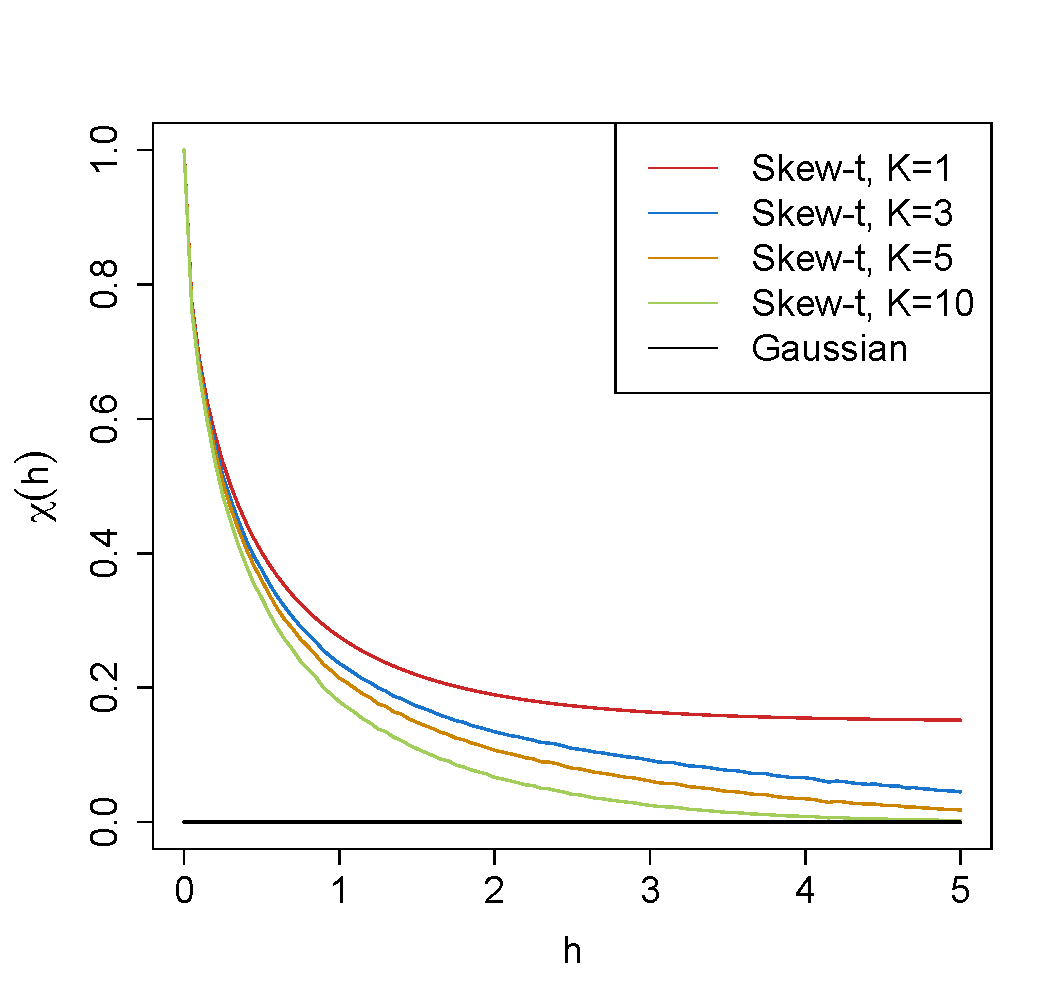
\includegraphics[width=0.5\linewidth]{plots/chi-h.pdf}
  \caption{Extremal dependence measure $\chi(h)$, as a function of distance, $h$, for $K = 1, 3, 5$, and $10$ knots.}
  \label{stfig:chi}
\end{figure}

\subsection{Extension to space-time data} \label{sts:temporal}
When using daily measurements, the assumption of temporal independence is often inappropriate.
In this section, we extend \eref{steq:partition} to the spatiotemporal setting.
There are several places where temporal dependence could be incorporated in the model, including the Gaussian process $v_t(\bs)$.
However, we choose to allow for temporal dependence in the $\bw$, $z$, and $\sigma$ terms because these terms dictate the tail behavior of the process which is our primary focus (see \aref{sta:temporal} for a discussion of the induced temporal asymptotic dependence).
Let
\begin{align} \label{steq:spatiotemp}
  Y_t(\bs) = \bX_t(\bs)^\top \bbeta + \lambda \sigma_t(\bs) |z_t(\bs)| + \sigma_t(\bs) v_t(\bs),
\end{align}
where $t \in \{1, \ldots, n_t\}$ denotes the day of each observation.
Let \hbox{$\bw_{tk} = (w_{tk1}, w_{tk2})$} be a spatial knot on day $t$, and let $\bw_{t1}, \ldots, \bw_{tK}$ be the collection of spatial knots on day $t$.
As in \sref{sts:part}, these knots define a daily partition $P_{t1}, \ldots, P_{tK}$, and for $\bs \in P_{tk}$,
\begin{align}
  z_t(\bs) = z_{tk}\quad \text{and} \quad \sigma_{t}(\bs) = \sigma_{tk}.
\end{align}
We allow the partition structure to vary from day to day in order to account for sharp spikes in a response that may not be present every day (e.g. the impact of a forest fire on ozone levels).

We use an AR(1) time series model for $\bw_{tk}$, $z_{tk}$, and $\sigma_{tk}$.
The time series model must be specified after a transformation to preserve the \skewt process at each time point.
For each time-varying parameter, we transform the parameter to obtain a standard normal marginal distribution, place a Gaussian prior with autocorrelation on the transformed parameter, and then transform back to the appropriate marginal distribution for the \skewt process.
We first transform the spatial knots from $\calD$ to $\mathbb{R}^2$ as follows.
Let
\begin{align} \label{steq:wstar}
  w^*_{tki} = \Phi^{-1}\left[ \frac{ w_{tki} - \min(\bs_i)}{ \max(\bs_i) - \min(\bs_i) } \right], \quad i = 1, 2
\end{align}
where $\Phi$ is a univariate standard normal density function and $\bs_i = [s_{1i}, \ldots, s_{ni}]$.
Then the transformed knots $\bw^*_{tk} \in \mathbb{R}^2$.
We use a transformation of a Gaussian random variable on $z_{t}(\bs)$ to ensure that the marginal distributions of $z_t(\bs)$ are half-normal.
Let
\begin{align} \label{steq:zstar}
  z^*_t(\bs) = \Phi^{-1}\left\{ \text{HN}[z_t(\bs)] \right\}
\end{align}
where HN is the distribution function of a half-normal random variable.
We also use a transformation of a Gaussian random variable on $\sigma^2_t(\bs)$ to ensure that the marginal distributions of $\sigma^2_t(\bs)$ are inverse gamma.
Let
\begin{align} \label{steq:sigmastar}
  \sigma^{2*}_t(\bs) =\Phi^{-1}\left\{ \text{IG}[\sigma^2_t(\bs)] \right\}
\end{align}
where IG is defined as before.
The AR(1) process for each tail parameter is $\bw^*_{1k} \sim N_2(\bZero, \bI_2)$ where $\bI_2 = \text{diag}(1, 1)$, $z^*_{1k} \sim N(0, 1)$, $\sigma^{2*}_{1k} \sim N(0, 1)$, and for $t > 1$ the time series is modeled as
\begin{align}
  \bw^*_{tk} | \bw^*_{t-1, k} &\sim N_2\left[\phi_w \bw^*_{t-1, k}, (1 - \phi_w^2) \bI_2 \right] \label{steq:ts-wstar}\\
  z^*_{tk} | z^*_{t-1, k} &\sim N \left[\phi_z z^*_{t-1, k}, (1 - \phi_z^2)\right] \label{steq:ts-zstar} \\
  \sigma^{2*}_{tk} | \sigma^{2*}_{t-1, k} &\sim N \left[\phi_\sigma \sigma^{2*}_{t-1, k}, (1 - \phi_\sigma^2) \right] \label{steq:ts-sigmastar}
\end{align}
where $|\phi_w|$, $|\phi_z|$, $|\phi_\sigma| < 1$.
These are stationary time series models with marginal distributions \hbox{$\bw^*_{k} \sim N_2(\bZero, \bI_2)$} \hbox{$z^*_{k} \sim N(0, 1)$}, and \hbox{$\sigma^{2*}_{k} \sim N(0, 1)$}.
After transformation back to the original space, $\bw_{tk} \sim \mathrm{Unif}(\calD)$, $z_{tk} \sim \mathrm{HN}(0, 1)$, and $\sigma^2_{tk} \sim \mathrm{IG}(a / 2, b / 2)$.
We then create the partition for day $t$ using $\bw_{t1}, \ldots, \bw_{tK}$.
For each day, the model is identical to the spatial-only model in \eref{steq:partition} by construction.

\section{Hierarchical model}\label{sts:hier}
We define a Bayesian hierarchical model based on the \skewt process and use a Markov chain Monte Carlo (MCMC) algorithm to fit the data.
We model our data as partially censored observations (see \sref{sts:censoring}) from the \skewt model defined in \sref{sts:spatial}.
In the first step of the MCMC algorithm, we impute censored values of $\widetilde{Y}$ such that the estimation of model parameters can be based on the completed $\bY$.
% We model our data as observations from the censored \skewt model defined in \sref{sts:censoring}.
Conditioned on $z_{tk}(\bs)$, $\sigma^2_{tk}(\bs)$, and $P_{tk}$, joint distribution of $\bY$ is multivariate Gaussian.
We do not fix the partitions; instead, the locations of the $K$ knots are treated as unknown and random.
% The first step in the algorithm is to update the knot locations, $z_{tk}(\bs)$, $\sigma^2_{tk}(\bs)$.
% The knot locations are treated as unknown and random in the MCMC algorithm.
% For level
%  $\bw_{t1}, \ldots, \bw_{tK}$ be a set of daily spatial knots in a spatial domain of interest, $\calD$, and $P_{tk}$ as defined in \eref{steq:subregions}.
One approach would be to allow $K$ to be unknown and follow a Poisson process prior, but this would lead to onerous computing.
Therefore, we elect to treat $K$ as a tuning parameter for the MCMC by fixing it at different values and assessing its impact on prediction as described in \sref{sts:modelselect}.
Then the hierarchical model is given as
\begin{align}
   Y_t(\bs) \mid z_{t}(\bs), \sigma_t^2(\bs), P_{tk}, \Theta &= \bX_t(\bs)^\top \beta + \lambda \sigma_t(\bs) |z_t(\bs)| + \sigma_t(\bs) v_t(\bs) \label{steq:hier}\\
   z_t(\bs) &= z_{tk} \text{ if } \bs \in P_{tk}\nonumber\\
   \sigma^2_{t}(\bs) &= \sigma^2_{tk} \text{ if } \bs \in P_{tk}\nonumber\\
   \lambda & \sim N(0, \sigma^2_\lambda)\nonumber \\
   % \lambda_1 &= \left\{ \begin{array}{ll}
   %    +1 \quad & \text{w.p. } 0.5\\
   %    -1 \quad & \text{w.p. } 0.5
   % \end{array}\right.\nonumber\\
   % \lambda^2_2 & \sim IG(a, b)\nonumber\\
   v_t(\bs) \mid \Theta &\sim \Matern(\bZero, \bSigma)\nonumber
\end{align}
% \begin{align*}
%    z^*_{tk} \mid z^*_{t-1, k} &\sim N(\phi_z z^*_{t-1, k}, (1 - \phi_z^2))\nonumber\\
%    \sigma^{2*}_{tk} \mid \sigma^{2*}_{t-1, k} &\sim N(\phi_\sigma \sigma^{2*}_{t-1, k}, (1 - \phi_\sigma^2))\nonumber\\
%    \bw^*_{tk} \mid \bw^*_{t-1, k} &\sim N_2(\phi_w \bw^*_{t-1, k}, \bI_2 (1 - \phi_w^2) ) \nonumber
% \end{align*}
where $\Theta = \{\varphi, \nu, \gamma\, \lambda, \bbeta\}$, $\bSigma$ is a \Matern covariance matrix as described in \sref{sts:skewt}, and the priors on $\bw^*_{tk}$, $z^*_{tk}$, and $\sigma^{2*}_{tk}$ are given in \eref{steq:ts-wstar} -- \eref{steq:ts-sigmastar}.

\subsection{Computation}\label{sts:comp}
We use MCMC methods to estimate the posterior distribution of the model parameters.
At each MCMC iteration, we first impute values below the threshold conditional on observations above the threshold.
% This is feasible for large datasets with our model because for a single day, conditional on the model parameters, we only need to draw from a truncated multivariate normal distribution.
% We can use Gibbs sampling to update $Y_t(\bs)$ for censored observations that are below the threshold $T$.
After conditioning on $\lambda$, $z_t(\bs)$ and non-censored observations, $Y_t(\bs)$ has truncated normal full conditionals $Y_t(\bs) \sim N_{(-\infty, T)}(\bX_t^\top(\bs) \beta + \lambda | z_t(\bs)|, \bSigma)$.

We update model parameters $\Theta$ using Gibbs sampling with Metropolis-Hastings steps when needed.
In our case, we also wish to be able to make predictions at sites where we do not have data.
We can easily implement Bayesian Kriging as a part of the algorithm to generate a predictive distribution for $Y_t(\bs^*)$ at prediction location $\bs^*$.
This step is similar to the imputation for censored observations except that the full conditionals are no longer truncated at $T$.
See Appendices A.1 and A.2 for details regarding the MCMC algorithm.

\section{Simulation study}\label{sts:simstudy}
In this section, we present the results from a simulation study to investigate how the number of partitions and the amount of thresholding impact the accuracy of predictions made by the model and to compare with Gaussian and max-stable methods.

\subsection{Design}\label{sts:simdesign}
For all simulation designs, we generated data from model \eref{steq:partition} in \sref{sts:part} using $n_s=144$ sites and $n_t=50$ independent days.
The sites were generated uniformly on the square $[0, 10] \times [0, 10]$.
We generated data from five different simulation designs:
\begin{enumerate}
  \item Gaussian, $K=1$ knot
  % \item Symmetric-$t$ marginal, $K=1$ knot
  % \item Symmetric-$t$ marginal, $K=5$ knots
  \item \Skewt, $K=1$ knots
  \item \Skewt, $K=5$ knots
  \item \citet{Reich2012} max-stable process %with GEV(1, 1, 0.2) marginals with dependence parameteter $\gamma_{\text{AL}} = 0.5$
  % \item Transformation below $T = q(0.80)$
  \item Brown-Resnick max-stable process \citep{Kabluchko2009} %with unit Fréchet marginals and stable semivariogram with range 1 and smoothness 0.5
\end{enumerate}
In the first three designs, the realizations from $v_t(\bs)$ were generated using a \Matern covariance with smoothness parameter $\nu = 0.5$, spatial range $\varphi = 1$ and $\gamma = 0.9$.
In the first design, $\sigma^2 = 2$ was used for all days which results in a Gaussian distribution.
For designs 2 and 3, $\sigma^2_{tk} \iid \text{IG}(3, 8)$ to give a $t$ distribution with 6 degrees of freedom.
For design 1, we set $\lambda = 0$.
For designs 2 and 3, $\lambda = 3$ was used as to simulate moderate skewness, and the $z_t$ were generated as described in \sref{sts:part}.
In designs 1 -- 3, the mean $\bX^\top \bbeta = 10$ was assumed to be constant across space.
In the fourth design, we generated from the max-stable model of \citet{Reich2012}.
The marginal distributions follow a generalized extreme value distribution with location parameter 1, scale parameter 1, and shape parameter 0.2.
Spatial dependence in the form an asymmetric logistic dependence function is induced by random effects for kernel basis functions associated with 144 spatial knots defined on a square grid on $[1,9] \times [1,9]$.
We set the dependence parameter ($\alpha$ in Reich and Shaby, 2012) to 0.5 which represents moderate spatial dependence.
For the final design, we generated data from a Brown-Resnick max-stable process  using \texttt{rmaxtab} in the \texttt{SpatialExtremes} package of \texttt{R} \citep{Ribatet2015}.
For this design we fixed unit \Frechet margins, and we used a range of 1 and smoothness 0.5.
% In the final design, we generate $\tilde{y}$ using the setting from design 2, and then transform the data
% \begin{align}
%   y = \left\{ \begin{array}{lc}
%     \tilde{y}, \quad & \tilde{y} > T \\[0.5em]
%     T \exp\{\tilde{y} - T\}, \quad & \tilde{y} \le T
%   \end{array}\right.
% \end{align}
% where $T = q(0.80)$ is the 80th sample quantile of the data.
% The final design is included to explore the importance of using a threshold exceedance model when the distribution for the bulk of the data is misspecified.

$M = 50$ data sets were generated for each design.
For each data set we fit the data using six models
\begin{enumerate}
  \item Gaussian marginal, $K=1$ knots
  \item \Skewt marginal, $K=1$ knots, $T=-\infty$
  \item Symmetric-$t$ marginal, $K=1$ knots, $T=q(0.80)$
  \item \Skewt marginal, $K=5$ knots, $T=-\infty$
  \item Symmetric-$t$ marginal, $K=5$ knots, $T=q(0.80)$
  \item \citet{Reich2012} max-table model thresholded at $T = q(0.80)$
\end{enumerate}
where $q(0.80)$ is the 80th sample quantile of the data.
All methods were fit using a fully-Bayesian approach that simultaneously estimates marginal and spatial dependence parameters.
The design matrix $\bX$ includes an intercept with a first-order spatial trend with priors of $\beta_\text{int}$, $\beta_\text{lat}$, $\beta_\text{long},  \iid \text{N}(0, 10)$ although only the intercept is used in the data generation.
The spatial covariance parameters have priors $\log(\nu) \sim \text{N}(-1.2, 1)$, $\gamma \sim \text{Unif}(0, 1)$, $\varphi \sim \text{Unif}(0, 15)$.
The skewness parameter has prior $\lambda \sim N(0, 20)$.
The residual variance terms have priors $\sigma^2_t(\bs) \sim \text{IG}(a / 2, b / 2)$, where $a$ has a discrete uniform prior on a mesh from $0.2$ to $20$ with spacing of $0.1$ and $b$ has a Gamma$(0.1, 0.1)$ prior.
As described in \sref{sts:skewt}, these priors are meant to be fairly uninformative to allow the data to dictate both the degrees of freedom $a$ and precision $b$ of the process.
The knots have priors $\bw \sim \text{Unif}(\calD)$.
We tried also fitting the \skewt marginals for the thresholded models, but it is very challenging for the MCMC to properly identify the skewness parameter with a censored left tail.
Each chain of the MCMC ran for 20,000 iterations with a burn-in period of 10,000 iterations.
Although the goal of this simulation study is not to assess parameter estimation, for design (2) and method (2) where data are generated and fit with a \skewt distribution, the samples converges for $\lambda$ and $a$, and the empirical coverage of posterior 95\% intervals is near the nominal level (96\% coverage for $\lambda$ and 90\% for $a$).
It should be noted that in the models with multiple partitions (i.e. models 4 and 5) it is hard to assess the convergence of $\bw$, $z(\bs)$, and $\sigma^2(\bs)$ because of partition label switching throughout the MCMC; however, we are not interested in these parameters but rather spatial predictions and tail probabilities which converge well.
Finally, we did not fit a Brown-Resnick model because we cannot use a Bayesian approach with so many sites.

\subsection{Cross validation}\label{sts:modelselect}
Models were compared using cross validation, with 100 sites used as training sites to fit the models, and 44 sites withheld for testing the predictions.
Because one of the primary goals of this model is to predict exceedances over a high level, we use Brier scores to compare the models \citep{Gneiting2007}.
The Brier score for predicting exceedance of a level $L$ is given by $[e(L) - P(L)]^2$ where $e(L) = I[y>L]$ is an indicator function indicating that a test set value, $y$, has exceeded the level, $L$, and $P(L)$ is the predicted probability of exceeding $L$.
We average the Brier scores over all test sites and days.
For the Brier score, a lower score indicates a better fit.

\subsection{Results}\label{sts:simresults}
We compared the Brier scores for exceeding four different high levels for each dataset.
The levels used for the Brier scores are extreme quantiles from the simulated data for $L = q(0.90)$, $q(0.95)$, $q(0.98)$, $q(0.99)$.
\fref{stfig:simbrierscores} gives the Brier score relative to the Brier score for the Gaussian method calculated as
\begin{align}
  \text{BS}_{\text{rel}} = \frac{\text{BS}_{\text{method}}}{\text{BS}_{\text{Gaussian}}}.
\end{align}
We analyzed the results for the simulation study using a Friedman \citep{Hollander2014} test at $\alpha = 0.05$ to see if at least one method had a significantly different Brier score.
For Friedman tests that came back with a significant p-value, we conducted a Wilcoxon-Nemenyi-McDonald-Thompson \citep{Hollander2014} test to see which of the methods had different results.
The full results for the Wilcoxon-Nemenyi-McDonald-Thompson tests are given in \aref{sta:pdiffs}.

In general, we find that when the method to fit the data matches the data generation scheme, there is some improvement over other methods.
The results show that when the data are generated from a Gaussian process, our method performs comparably to a Gaussian approach.
In general, when the underlying process is not Gaussian, our method results in an improvement over both the max-stable and Gaussian methods.
We also see that the non-thresholded methods tend to outperform the thresholded methods, but this is not surprising given that in most cases, the data are generated directly from the model.
Finally, in the case where the data are generated from a Brown-Resnick process, we find that our method is competitive with using a max-stable model.
% Finally, for setting 5, although the thresholded version of the single-partition model tends to perform the best across all of the extreme quantiles, the difference between the thresholded and non-thresholded methods is no longer significant in the more extreme quantiles.
In summary, our method provides great flexibility for data that demonstrate some level of asymmetry and heavy tails, while still performing comparably to Gaussian methods when the data are symmetric and have light tails.

\begin{figure}
  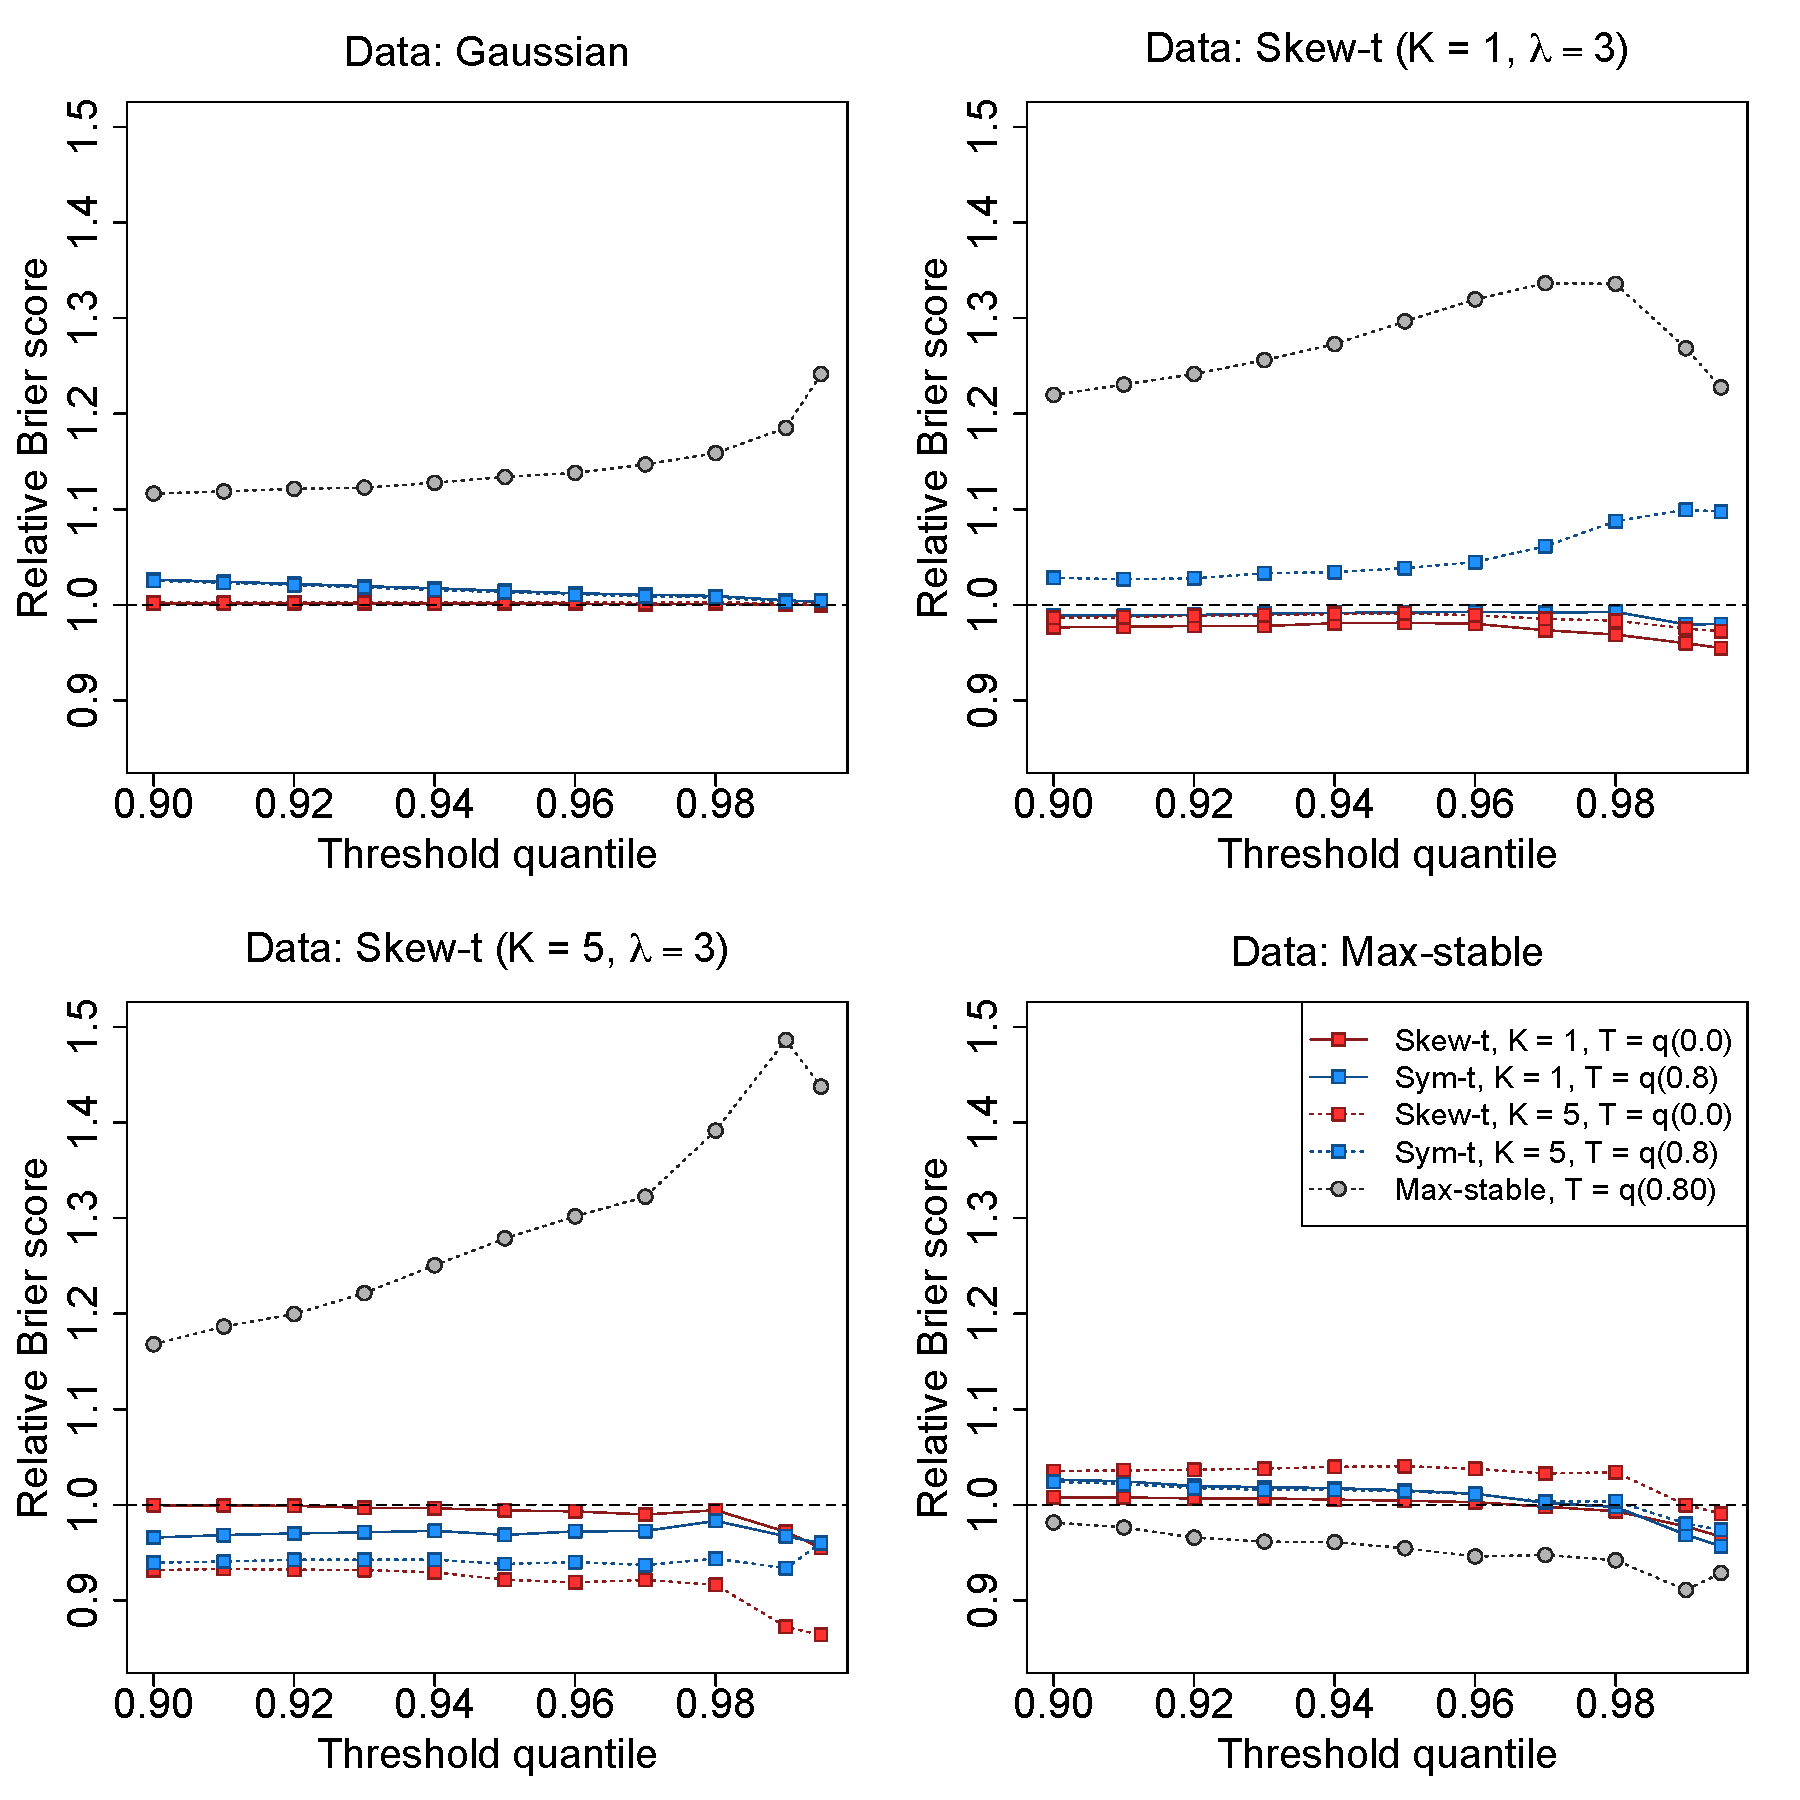
\includegraphics[width=\linewidth]{plots/bsplots-mean.pdf}
  \caption{Brier scores relative to the Gaussian method for simulation study results. A ratio lower than 1 indicates that the method outperforms the Gaussian method.}
  \label{stfig:simbrierscores}
\end{figure}

\section{Data analysis}\label{sts:analysis}
We consider daily observations of maximum 8-hour ozone measurements for the 31 days of July 2005 at 1,089 Air Quality System (AQS) monitoring sites in the United States as the response (see \fref{stfig:ozone-10jul}).
For each site, we also have covariate information containing the estimated ozone from the Community Multi-scale Air Quality (CMAQ) modeling system.
Initially, we fit a linear regression with $\bX_t(\bs) = [1, \text{CMAQ}_t(\bs)]^\top$. % assuming a mean function of
% \begin{align}
%   \text{E}[Y_i(\bs)] = \beta_0 + \beta_1 \cdot \text{CMAQ}_t(\bs). \label{steq:datamean}
% \end{align}
\fref{stfig:ozone-qq} shows a Q-Q plot of the residuals compared to a \skewt distribution with $a = 10$ and $\lambda = 1$, suggesting the data are heavy tailed.
\begin{figure}
  \centering
  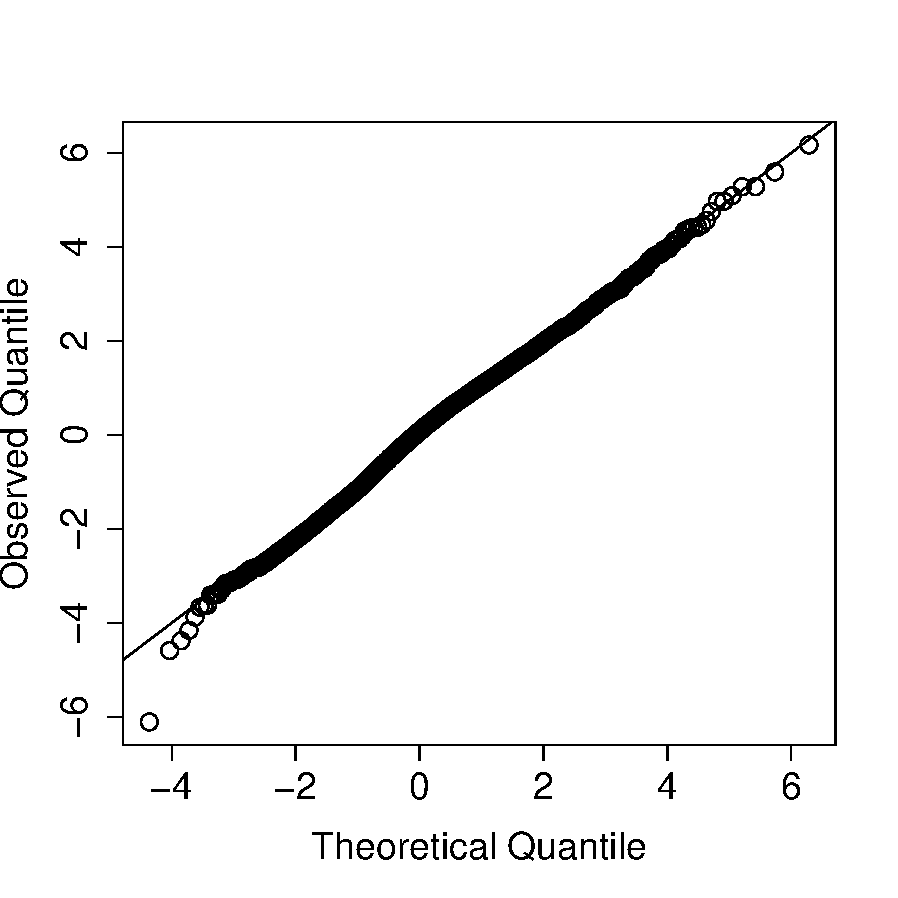
\includegraphics[width=\linewidth]{plots/qq-res.pdf}
  \caption{Gaussian Q-Q plot (left) and \skewt with $a = 10$ and $\lambda = 1$ Q-Q plot (right) of the residuals.}
  \label{stfig:ozone-qq}
\end{figure}

Standard exploratory data analysis techniques for extremal dependence are very challenging with only 31 days worth of data because it is difficult to estimate extreme quantiles at each site to obtain empirical estimates of $\chi$.
Despite the fact that there is only one month of data, we can get some sense of extremal dependence between sites by looking at joint occurrences of high sample quantiles.
For example, \fref{stfig:bivariateozone} suggests there is more agreement between sites that are close to one another than sites that are far from one another.
\begin{figure}
  \centering
  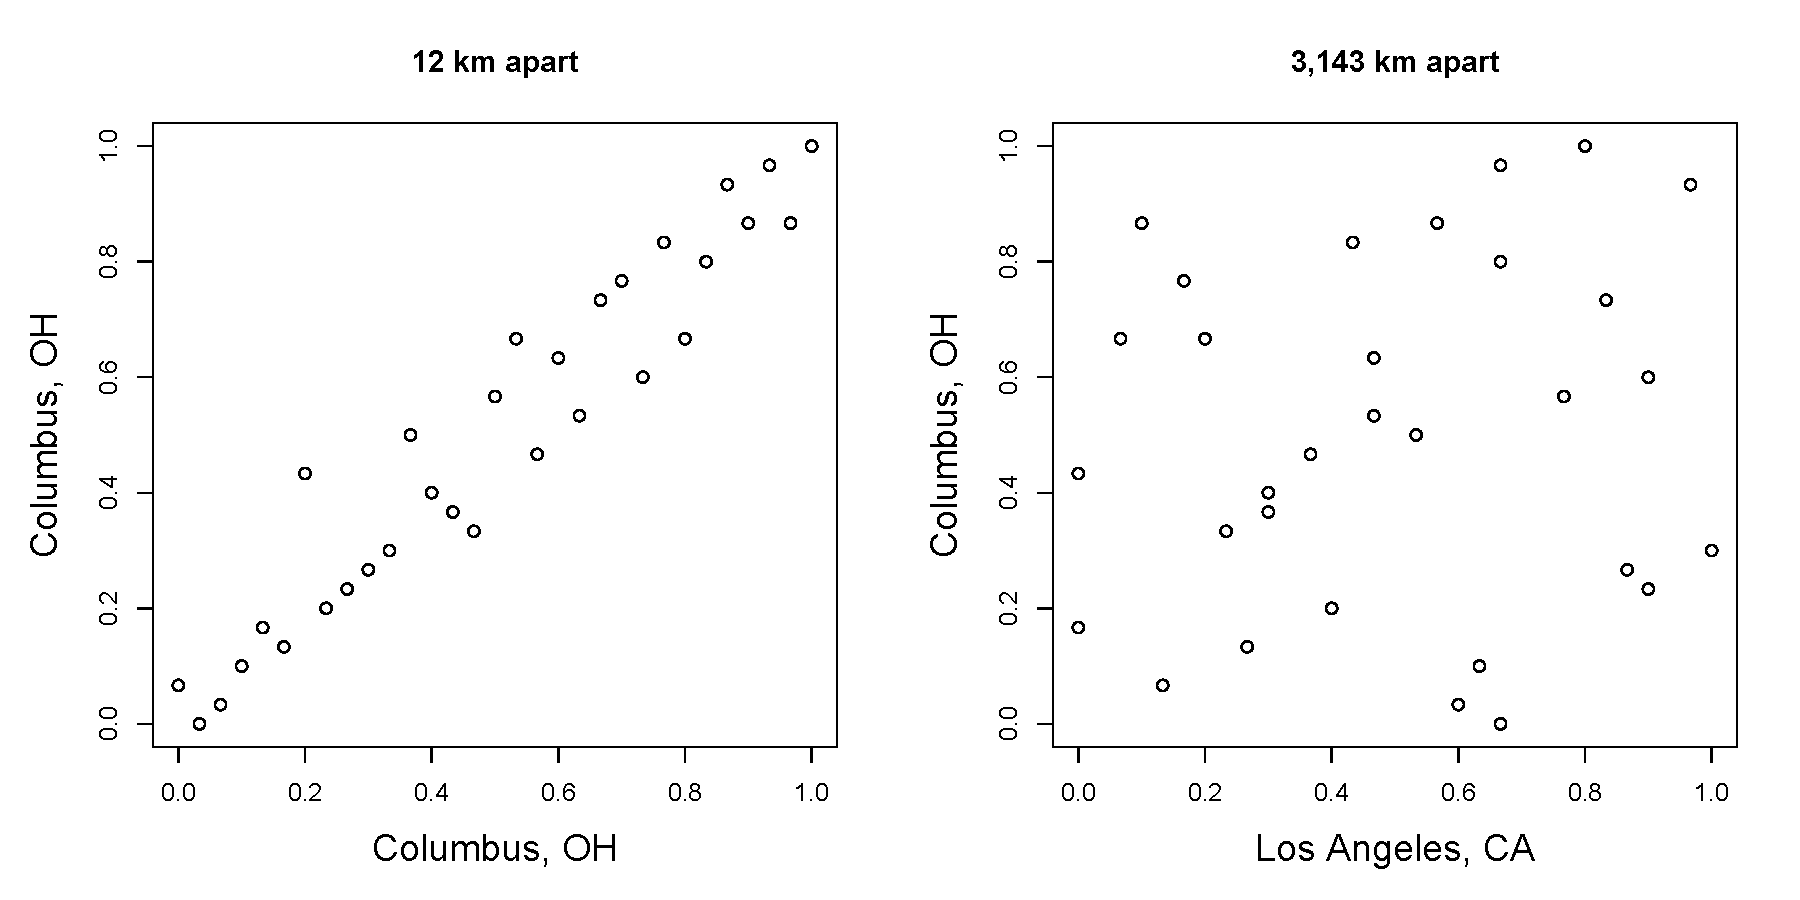
\includegraphics[width=\linewidth]{plots/daily-quantiles-ozone.pdf}
  \caption{Daily quantiles for two monitoring locations near Columbus, OH (left) and daily quantiles for a monitoring location in Los Angeles, CA and Columbus, OH (right)}
  \label{stfig:bivariateozone}
\end{figure}
% Another aspect that distinguishes our approach from more traditional extremes analyses, is how the threshold is selected.
% In our example, a threshold of 75 ppb which corresponds to $q(92)$ for all observations, but marginally it represents anywhere from $q(0.06)$ to $q(1)$.

% We explore spatial and temporal extremal dependence by considering $\chi_c = \Pr[Y(\bs) > c | Y(\bt) > c]$.
% To examine spatial dependence in high quantiles, we consider observations at all pairs of sites $\bs$ and $\bt$ that are distance $h$ apart where $h$ is separated into bins of size 0.25 km.
% Then conditioned on $Y(\bt) > c$, we take the sample proportion of $Y(\bs) > c$.
% Finally, $\widehat{\chi}_c(h)$ is averaged over all days at each of the three threshold quantiles.
% To examine temporal dependence in high quantiles, we consider observations at a single site that are taken lag-$t$ days apart.
% Then conditioned on $Y_n(\bs) > c$, we take the sample proportion of $Y_{n + t}(\bs) > c$.
% Finally, $\widehat{\chi}(t)$ is averaged over all sites at each of the three threshold quantiles.
% The $\widehat{\chi}_c(h)$ and $\widehat{\chi}_c(t)$ plots in Figure \ref{ststfig:chi-st} show the estimated spatial and temporal dependence of the residuals for the ozone data at three quantile levels $q(0.90), q(0.95)$, and $q(0.99)$.

% \begin{figure}
%   \centering
%   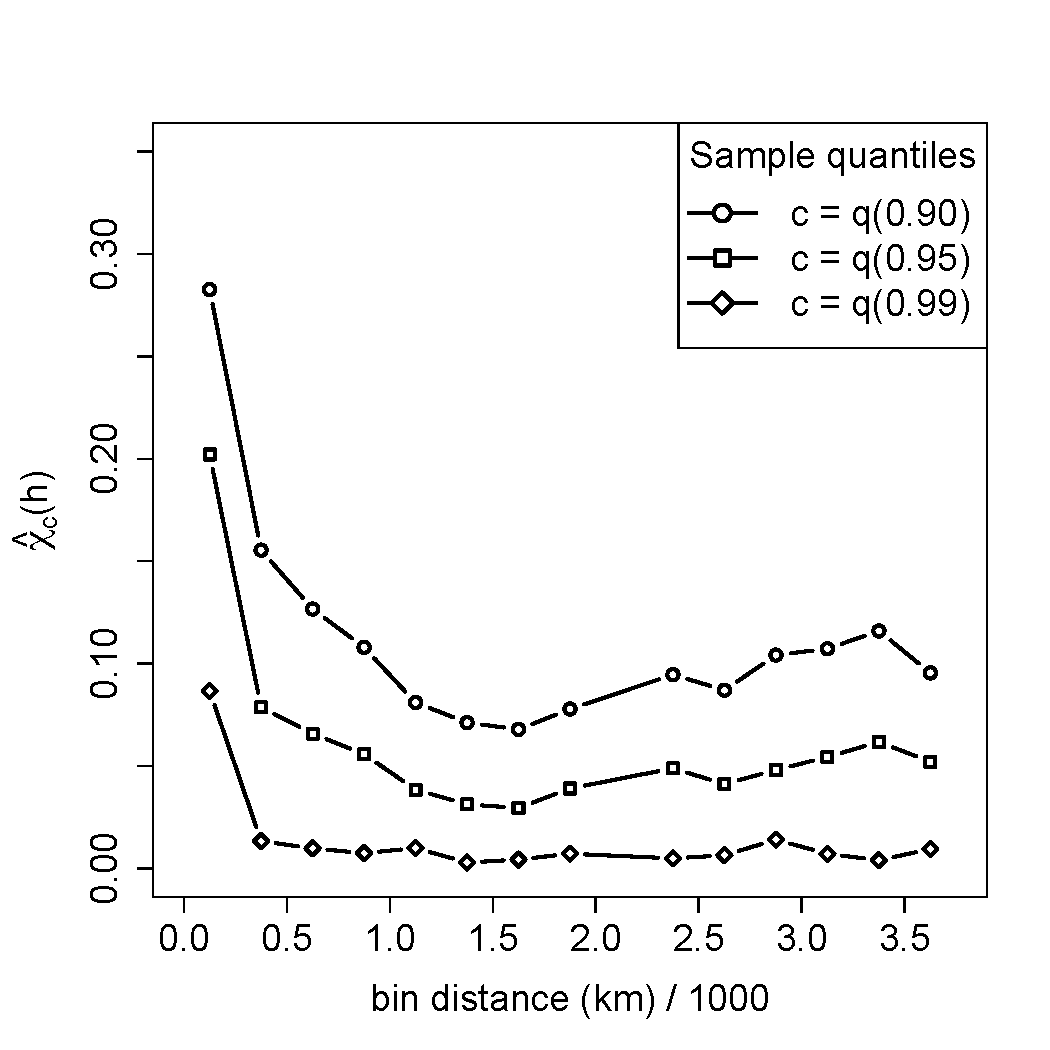
\includegraphics[width=0.49\linewidth]{plots/chi-h-ozone.pdf}
%   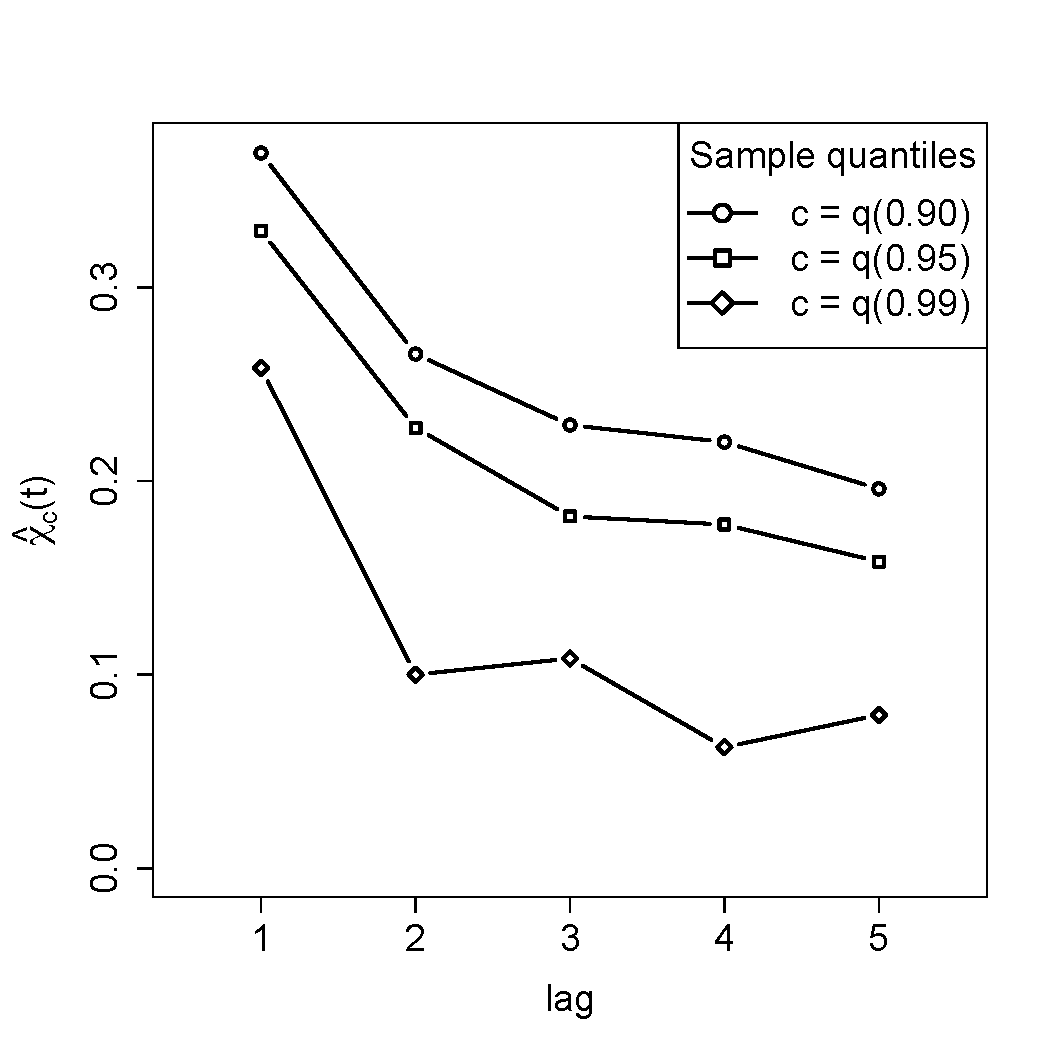
\includegraphics[width=0.49\linewidth]{plots/chi-t-ozone.pdf}
%   \caption{$\widehat{\chi}_c(h)$ plot for the residuals (left). $\widehat{\chi}_c(t)$ plot for the residuals (right).}
%   \label{stfig:chi-st}
% \end{figure}

\subsection{Model comparisons}
We fit the model using Gaussian and \skewt marginal distributions with $K=1, 5, 6, 7, 8, 9, 10, 15$ partitions.
We censored $Y(\bs)$ at $T = 0$, $T = 50$ (0.42 sample quantile), and $T = 75$ (0.92 sample quantile) ppb in order to compare results from no, moderate, and high censoring.
The upper threshold of 75 ppb was used because the current air quality standard is based on exceedance of 75 ppb.
As with the simulation study, for models with a threshold of $T = 75$, we used a symmetric-$t$ marginal distribution.
We also compared models with no time series to models that included the time series.
Finally, as a comparison to max-stable methods, we fit the model using the hierarchical max-stable model of \citet{Reich2012} with the data thresholded at $T = 75$.
All methods assumed $\bX_t(\bs) = [1, \text{CMAQ}_t(\bs)]^\top$.
To ensure that the max-stable method ran in a reasonable amount of time, we used a stratified sub-sample of 800 sites.
We conducted two-fold cross validation using 400 training sites and 400 validation sites as described in \sref{sts:modelselect}

Each chain of the MCMC ran for 30,000 iterations with a burn-in period of 25,000 iterations.
We used the same priors for the spatial covariance parameters, skewness parameter, and knots as in the simulation study.
The prior for the residual variance terms was $\sigma^2_t(\bs) \sim \text{IG}(a / 2, b / 2)$ where $a$ was the same as the simulation study, but $b$ had a Gamma$(1, 1)$ prior.
Parameters appeared to converge properly; however, as before, for models with multiple partitions it was hard to assess the convergence of $\bw$, $z(\bs)$, and $\sigma^2(\bs)$ because of partition label switching throughout the MCMC.
For each model, we averaged Brier scores over all sites and days to obtain a single Brier score for each dataset.
At a particular level, the model that fit the best was the one with the lowest score.
We then computed the relative (to Gaussian) Brier scores (see \sref{sts:simresults}) to compare each model.

\subsection{Results}\label{sts:results}
The results suggest that the \skewt, thresholded, partitioned, and time series models all give an improvement in predictions over the Gaussian model, whereas the max-stable method results in relative Brier scores between 1.13 and 1.18 indicating poorer performance than the Gaussian model.
The plots in \fref{stfig:bs-ozone} show the relative Brier scores for time-series and non-time-series models, using $K = $ 1, 7, and 15 knots at thresholds $T = $ 0, 50, and 75 ppb.
Most of the models perform similarly across all the Brier scores; however, for single-partition models without thresholding, performance tends to diminish in the extreme quantiles.
The results also suggest that thresholding improves performance for estimates in the extreme quantiles.
Both plots have similar features suggesting that most settings do reasonably well.
In particular, for all extreme quantiles, selecting a moderate number of knots (e.g. $K = 5, \ldots, 10$) tends to give the best results.
\tref{sttbl:ozoneresults} shows the best two models for selected extreme quantiles.

We illustrate the predictive capability of our model in \fref{stfig:ozoneq99} by plotting the 99th quantile for South Carolina and Georgia, a subset of the spatial domain, in order to study local features.
The four methods used are
\begin{enumerate}
  \item Gaussian
  \item \Skewt, $K =$ 1 knot, $T = $ 0, no time series
  \item \Skewt, $K =$ 5 knots, $T = $ 50, no time series
  \item Symmetric-$t$, $K =$ 10 knots, $T = $ 75, time series.
\end{enumerate}
In the bottom two plots, we plot the differences between method 4 and methods 1 and 2.
The most noticeable differences between the reference methods and the comparison methods is that the comparison methods tend to give higher estimates of the 99th quantile along the I-85 corridor between Charlotte and Atlanta.
Among these methods, the fourth method demonstrates the best performance.
For a map of Brier scores for the 99th quantile between Gaussian and the fourth method, see \aref{sta:ozonesite}.

\begin{figure}
  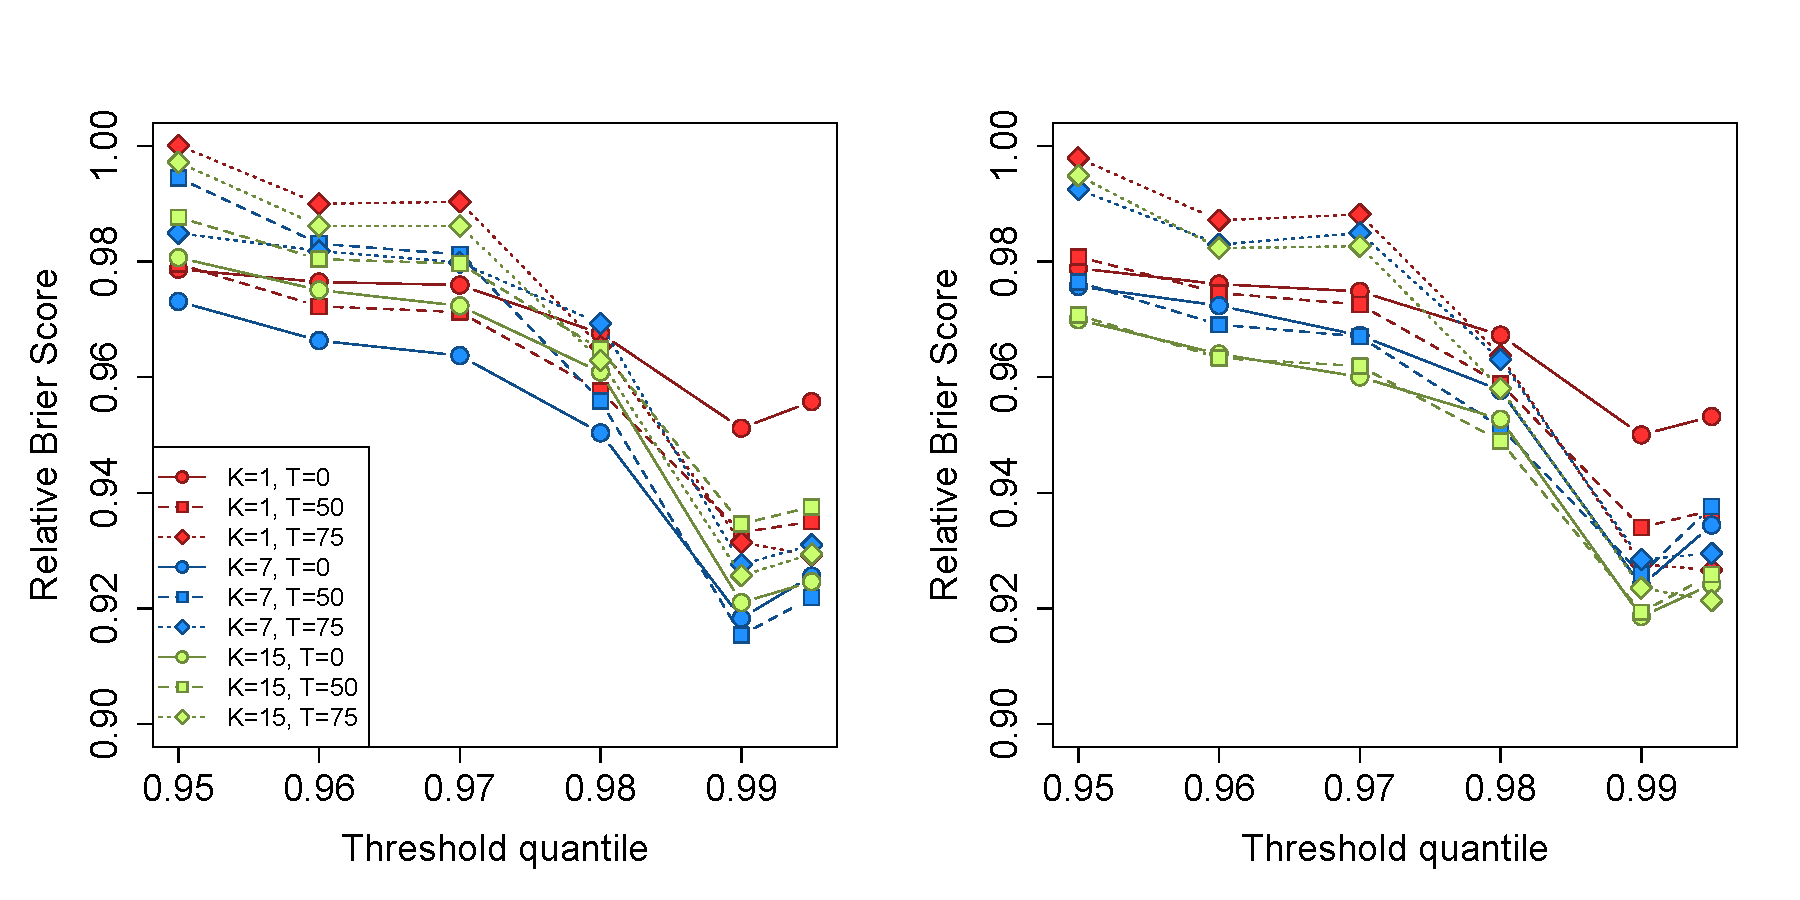
\includegraphics[width=\linewidth]{plots/bs-ozone.pdf}
  \caption{Relative Brier scores for time-series models (left) and non-time-series models (right). Relative brier score for the max-stable model is between 1.13 and 1.18}
  \label{stfig:bs-ozone}
\end{figure}
\begin{table}
  \scriptsize
  \caption{Top two performing models for predicting ozone exceedance of level $L$ with Relative Brier score}
  \label{sttbl:ozoneresults}
  \centering
  \begin{tabular}{l c l l l c c l l l c}
    \toprule
     \multicolumn{1}{c}{$L$} &\phantom{ab} & \multicolumn{4}{c}{1st} & \phantom{a} & \multicolumn{4}{c}{2nd} \\
    \cmidrule{1-1} \cmidrule{3-6} \cmidrule{8-11}
    $q(0.90)$  && No time series & $K=6$  & $T=50$  & BS: 0.992 &&
                 No time series & $K=1$  & $T=0$  & BS: 0.992 \\
    $q(0.95)$  && Time series & $K=5$ & $T=50$ & BS: 0.988 &&
                 No time series & $K=6$  & $T=50$ & BS: 0.989\\
    $q(0.98)$  && Time series & $K=7$  & $T=50$ & BS: 0.973 &&
                 Time series & $K=5$ & $T=50$ & BS: 0.975\\
    $q(0.99)$  && No time series    & $K=8$ & $T=0$ & BS: 0.946 &&
                 Time series    & $K=9$  & $T=75$ & BS: 0.947\\
    $q(0.995)$ && No time series    & $K=8$  & $T=0$ & BS: 0.951 &&
                 Time series    & $K=9$ & $T=75$ & BS: 0.956\\
    \bottomrule
  \end{tabular}
\end{table}

\begin{figure}
  \centering
  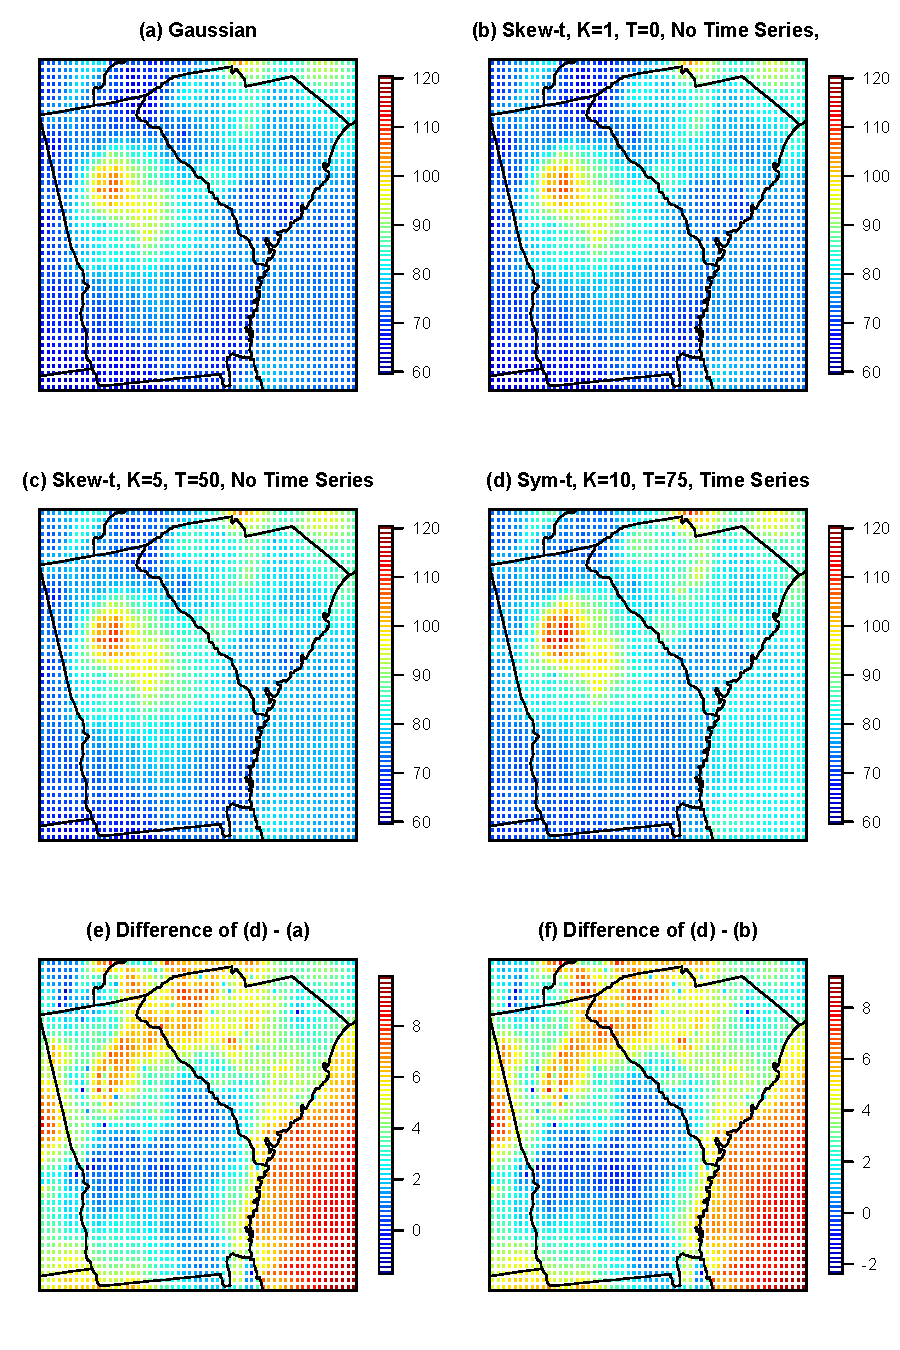
\includegraphics[height=0.95\textheight]{plots/q99-ozone.pdf}
  \caption{Panels (a) -- (d) give the posterior predictive $\widehat{q}(0.99)$ for the month of July under four different models, panel (e) gives the difference between $\widehat{q}(0.99)$ in panels (d) and (a), panel (f) gives the difference between $\widehat{q}(0.99)$ in panels (d) and (b).}
  \label{stfig:ozoneq99}
\end{figure}

\section{Discussion}\label{sts:con}
In this paper we propose a new threshold exceedance approach for spatiotemporal modeling based on the \skewt process.
The proposed model gives flexible tail behavior, demonstrates asymptotic dependence for observations at sites that are near to one another, and has computation on the order of Gaussian models for large space-time datasets.
In the simulation study, we demonstrate that this model shows statistically significant improvements over a na\"{i}ve Gaussian approach and in most cases, a max-stable approach.
In both the simulation study, and the application to ozone data, we find that incorporating a partition in the model can improve extreme predictions.
Furthermore the results from the data analysis suggest that thresholding can improve performance when predicting in the extreme tails of the data.

This model presents new avenues for future research.
One possibility is the implementation of a different partition structure.
We choose to define the random effects for a site by using an indicator function based on closeness to a knot.
However, this indicator function could be replaced by kernel function that would allow for multiple knots to impact each site, with the weight of each knot to be determined by some characteristic such as distance.
Another area that should be explored is the temporal dependence in the model.
Instead of implementing a time series on the random effects, a three-dimensional covariance structure on the residuals could be implemented to address temporal dependence.
Finally, we acknowledge that by specifying the number of knots, we may be underestimating the uncertainty in the model.
This could be incorporated by treating the number of knots as a model parameter instead of fixing it to be a specific value.
